\documentclass[12pt,a4paper]{article}

% Margins.
\setlength{\oddsidemargin}{0in}
\setlength{\evensidemargin}{0in}
\setlength{\headheight}{12pt}
\setlength{\headsep}{42pt}
\setlength{\topmargin}{-54pt}
\setlength{\textwidth}{6.5in}
\setlength{\textheight}{10in}

\usepackage{amsmath}
\usepackage{float}
\usepackage{graphicx}
\usepackage[hyphens]{url}
\usepackage{hyperref}	% Clickable links to figures, references and urls.
\usepackage{datetime}
\usepackage{subfigure}

% Links direct to top of figures.
\usepackage[all]{hypcap}

% Drawing.
\usepackage{pgf}
\usepackage{tikz}

% Listings for formatting code.
\usepackage{listings}
\usepackage{textcomp}
% General options.
\lstset{breaklines=true, basicstyle=\small\ttfamily, tabsize=4, numbers=left, stepnumber=1, frame=single, showstringspaces=false, upquote=true}
% C++ specific high-lighting. Comments are 50/50 shades of green/black and strings coloured with 60/40 red/black mixture.
\lstset{language=[ISO]C++, commentstyle=\color{green!50!black}, keywordstyle=\color{blue}, stringstyle=\color{red!60!black}}

%opening
\title{\vspace{-3cm}Physics for Engineers\\Assignment 09\\Ampere and Faraday's Laws}
\author{Arshad Hassan\and Attique Dawood}
\date{November 29, 2013\\Due: December 06, 2013\\[0.2cm] Last Modified: \today, \currenttime}
\begin{document}
\maketitle
\noindent\textbf{Question 1} A wire of radius $0.1$ cm carries $5$ mA current. Find current density.\\[0.2cm]
\noindent\textbf{Question 2} A coaxial wire of inner radius $\rho<0.1$ cm carries $I=10$ mA current. The outer conductor exists at $0.2<\rho<0.25$ cm and carries 10 mA return current. Find current densities in inner and outer conductor.\\[0.2cm]
\noindent\textbf{Question 3} A very thin infinite wire carries current $I$. Use Ampere's Law to find \textbf{H}.\\[0.2cm]
\noindent\textbf{Question 4} Use Ampere's Law to find \textbf{H} everywhere for wires in questions 1 and 2.\\[0.2cm]
\noindent\textbf{Question 5 \cite[Problem 7.21, page 300]{Sadiku}} An infinitely long filamentary wire carries 2 A current in $+z$ direction. Find
\begin{itemize}
\item[a.] \textbf{B} at (-3, 4, 7)
\item[b.] Magnetic flux through the surface given by $2<\rho<6$, $0<z<4$ and $\phi=90^0$.
\end{itemize}
\noindent\textbf{Question 6} A magnetic field given by $\textbf{B}=10\sin t\hat z$ cuts a current carrying loop. The loop is placed in $xy$--plane centred at $z$--axis and has a radius 5 cm. Find $V_{emf}$ and direction of induced current. What is induced current if current limiting resistor is 1 $\Omega$?\\[0.2cm]
\noindent\textbf{Question 7 \cite[Problem 9.4, page 404]{Sadiku}} A magnetic field given by $\textbf{B}=40\cos 10^4 t\hat z$ mW/m$^2$ cuts a current carrying loop. The loop is placed in $xy$--plane and has an area 20 cm$^2$. Find $V_{emf}$ and direction of induced current. What is induced current if current limiting resistor is 4 $\Omega$?\\[0.2cm]
\noindent\textbf{Question 8} A parallel--plate capacitor with plate area of 12 cm$^2$ and plate separation of 1 mm has an electric field $\textbf{E}=10\sin 1000t$ V/m applied across its plates. If the capacitor dielectric is $\epsilon=5\epsilon_0$ find the displacement current flowing through the capacitor. Also find capacitance. Repeat this problem if $\textbf{E}=20t$ V/m.\\[0.2cm]
\noindent\textbf{Question 9 \cite[Example 8.14, page 350]{Sadiku}} The toroidal core of figure \ref{Toroid-and-equivalent-circuit} has $\rho_0$ = 10 cm and a circular cross section with $a=1$ cm. If the core is made of steel ($\mu = 1000\mu_0$) and has a coil with 200 turns, calculate the amount of current that will produce a flux of 0.5 mWb in the core. Assume magnetic flux in the toroid is constant by taking $\rho_0>>a$.\\
\textbf{Answer:} 3.979 A.
\begin{figure}[H]
\centering
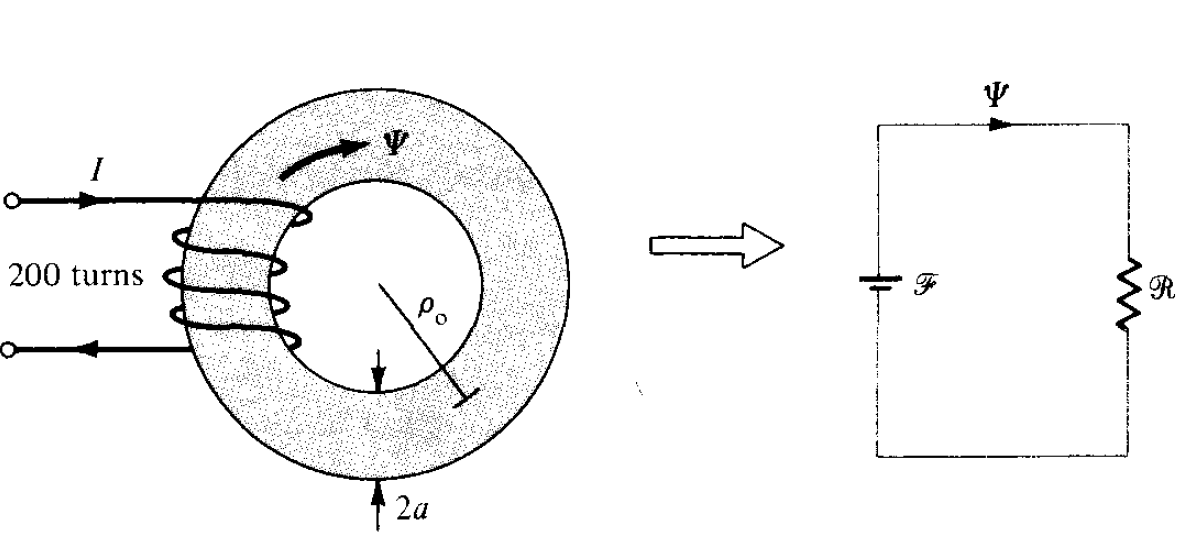
\includegraphics[scale=0.4]{Figure8-26S.png}
\caption{Toroid and equivalent magnetic circuit.}
\label{Toroid-and-equivalent-circuit}
\end{figure}
\bibliographystyle{plain}
\bibliography{PhysicsRef}
\end{document}
